\documentclass{beamer}

\usepackage{graphicx}
\usepackage{hyperref}
\usepackage{amsmath}

\usetheme{Darmstadt}
\usefonttheme[onlylarge]{structurebold}
\setbeamerfont*{frametitle}{size=\normalsize,series=\bfseries}
\setbeamertemplate{navigation symbols}{}

\usepackage{tikz}
\usetikzlibrary{arrows,shapes}
\usetikzlibrary{calc,decorations.pathmorphing,patterns}
\tikzstyle{block}=[draw opacity=0.7,line width=1.4cm]

\definecolor{lightpink}{rgb}{.96,.86,.86}
\definecolor{lightgreen}{rgb}{.86,.96,.86}

%I got the next chunk here https://tex.stackexchange.com/questions/109159/crossing-out-whole-slide-with-latex-beamer as a 
%solution for putting a big x across the whole slide
\makeatletter
\pgfdeclaredecoration{penciline}{initial}{
    \state{initial}[width=+\pgfdecoratedinputsegmentremainingdistance,auto corner on length=1mm,]{
        \pgfpathcurveto%
        {% From
            \pgfqpoint{\pgfdecoratedinputsegmentremainingdistance}
                            {\pgfdecorationsegmentamplitude}
        }
        {%  Control 1
        \pgfmathrand
        \pgfpointadd{\pgfqpoint{\pgfdecoratedinputsegmentremainingdistance}{10pt}}
                        {\pgfqpoint{-\pgfdecorationsegmentaspect\pgfdecoratedinputsegmentremainingdistance}%
                                        {\pgfmathresult\pgfdecorationsegmentamplitude}
                        }
        }
        {%TO 
        \pgfpointadd{\pgfpointdecoratedinputsegmentlast}{\pgfpoint{8pt}{5pt}}
        }
    }
    \state{final}{}
}

\newcommand{\var}{{\operatorname{var}}}
\newcommand{\cov}{{\operatorname{cov}}}
\newcommand{\cor}{{\operatorname{cor}}}
\newcommand{\E}{{\operatorname{E}}}
\newcommand{\mean}{{\operatorname{mean}}}
\newcommand{\cosp}{{\operatorname{cosp}}}

\title[Wavelet approaches to synchrony]
{
wsyn: Wavelet approaches to studies of synchrony in ecology
}

\author[Reuman]
{
D.C.~Reuman\inst{1} \\
J.A.~Walter\inst{2}
}

\institute
{
\inst{1}
University of Kansas \\
\inst{2}
UC Davis and University of Virginia
}

\date[KPT 2003]
{
May, 2024
}

\begin{document}

\begin{frame}
\titlepage
\end{frame}

\section{Introduction}

%In this Intro, we probably better put some of the caveating and provisors and citations
%we are presently putting into our review. This is not the only way to consider timescale
%specificity of synchrony, there is lots of other work on the subject, would be good
%to respect some of that work before going on with our way of doing it. 
%Maybe could have an example from an old Fourier paper (not even looking at synchrony) - timescale-specific methods have been used in ecology forever
%Maybe have an example of a "precursor study" or two where you can see they are talking about timescale-specific things. And maybe also changes through time (mention a couple early papers showing changes in synchrony). 
%Through decades of work by many researchers, the field has matured, helped at every stage by 1) long time series, and 2) ever improving statistical methods. This is one reasonably complete suite of such methods, but other authors use variant methods and so on which are also good and also allow us to learn about ecosystems.
%And the methods all overlap, being based on now-standard standard wavelet tools, differing in details we won't go into 
%Mention some of the other authors. 
%Our way of thinking about methods has been implemented in wsyn

\section{wsyn and synthetic examples}

%Somewhere above here you need to say the viewpoint is operational, i.e.,
%we talk about what these tools can get you and how you intepret it. Main ideas. 
%No time for detailed math, but we can provide some references if you want. 

%We should probably have a "reference" section in the github where we put:
%1) Torrence and Compo
%2) Some of our papers
%3) The wsyn vignette pdf
%3) A longer reference list

%You also want to mention, Dan, that the codes for this are in the github for the 
%seminar, and these are abbreviated from the vignette, so you have those two 
%resources, the latter in greater depth than what I have time for here.

\subsection{Wavelet transform}

{\setbeamercolor{background canvas}{bg=lightpink}
\begin{frame}
\frametitle{The wavelet transform}
\begin{itemize}
\item All the tools we discuss today are based on the wavelet transform
\item So we start by introducing it
\item Data consist of one time series
\end{itemize}
\end{frame}}

\begin{frame}
\frametitle{How to use the wavelet transform}
\begin{itemize}
\item Given a time series $x(t)$, the wavelet transform, $W_{\sigma}(t)$ is a complex number with:
\begin{itemize}
\item magnitude the strength of oscillation in $x(t)$ at time $t$ and timescale $\sigma$
\item phase the phase of that oscillation
\end{itemize}
\item So it decomposes variation by timescale, and tells you how that changes through time
\item You could also think of it as a time-windowed Fourier transform (but done correctly)
\end{itemize}
\end{frame}

\begin{frame}[fragile]
\frametitle{Example of wavelet transform: make some data}
\begin{block}{Fake data characteristics}
\begin{itemize}
\item One time series, sin wave of period 15, then switches to 8...
\item Plus white noise
\end{itemize}
\end{block}
\begin{exampleblock}{Make some fake data}
\begin{verbatim}
time1<-1:100; time2<-101:200; times<-c(time1,time2)

ts1<-c(sin(2*pi*time1/15),0*time2) #starts period 15
ts2<-c(0*time1,sin(2*pi*time2/8)) #then period 8
ts3<-rnorm(200,mean=0,sd=0.5) #add some white noise

ts<-ts1+ts2+ts3 
\end{verbatim}
\end{exampleblock}
\end{frame}

\begin{frame}[fragile]
\frametitle{Example of wavelet transform: apply \texttt{wsyn::wt}}
\begin{exampleblock}{Apply \texttt{wt}}
\begin{verbatim}
ts<-wsyn::cleandat(ts,times,clev=1)$cdat
wtres<-wsyn::wt(ts$cdat,times)
\end{verbatim}
\end{exampleblock}
\begin{block}{Notes}
\begin{itemize}
\item \texttt{cleandat} demeans time series (can also do more)
\item \texttt{wtres} is an S3 class defined for wavelet transforms
\item Default values for other \texttt{wt} arguments are good for exploration
\end{itemize}
\end{block}
\end{frame}

\begin{frame}[fragile]
\frametitle{Example of wavelet transform: what do you get?}
\begin{exampleblock}{Plot magnitude and phase}
\begin{verbatim}
wsyn::plotmag(wtres)
wsyn::plotphase(wtres)
\end{verbatim}
\end{exampleblock}
\includegraphics[width=.49\textwidth]{../results/synthetic_results/WaveletExample_magnitude.pdf}
\includegraphics[width=.49\textwidth]{../results/synthetic_results/WaveletExample_phase.pdf}
\end{frame}

\begin{frame}
\frametitle{Wavelet transform example}
\begin{columns}[c]
\begin{column}{6cm}
\begin{itemize}
\item The wavelet magnitude shows periodicity and change therein
\item A power spectrum would just show two peaks at timescales 8 and 15, no time resolution
\end{itemize}
\end{column}
\begin{column}{6cm}
\includegraphics[width=\textwidth]{../results/synthetic_results/WaveletExample_magnitude.pdf}
\end{column}
\end{columns}
\end{frame}

{\setbeamercolor{background canvas}{bg=lightgreen}
\begin{frame}
\frametitle{Advantages of the wavelet transform}
\begin{itemize}
\item Not only shows how the overall variability of the time series decomposes by timescale...
\item Also shows how that changes through time
\end{itemize}
\end{frame}}

\subsection{Time and timescale structure of synchrony}

{\setbeamercolor{background canvas}{bg=lightpink}
\begin{frame}
\frametitle{Displaying how synchrony depends on time and timescale}
\begin{itemize}
\item This talk covers an approach to exploring how synchrony depends on timescale...
\item and how it changes through time
\item So we next introduce methods for displaying the time and timescale structure of synchrony
based on the wavelet transform
\item Data now consist of multiple time series from different locations
\end{itemize}
\end{frame}}

\begin{frame}
\frametitle{The wavelet phasor mean field (\texttt{wsyn::wpmf})}
  \begin{itemize}
    \item For timeseries $x_n(t)$ in $n=1,\ldots,N$ locations
    \item For wavelet transforms $W_{n,\sigma}(t)$
    \item The WPMF is $\frac{1}{N} \sum_n \frac{W_{n,\sigma}(t)}{|W_{n,\sigma}(t)|}$
    \item In other words average the ``phasors'' $p_{n,\sigma}(t)= \frac{W_{n,\sigma}(t)}{|W_{n,\sigma}(t)|}$
    \item A ``phasor'' is a unit-magnitude complex number
    \item It gives phase synchrony as a function of time and timescale
  \end{itemize}
\end{frame}

\begin{frame}
  \frametitle{The wavelet phasor mean field - gives a detailed picture of synchrony}
  \begin{center}
    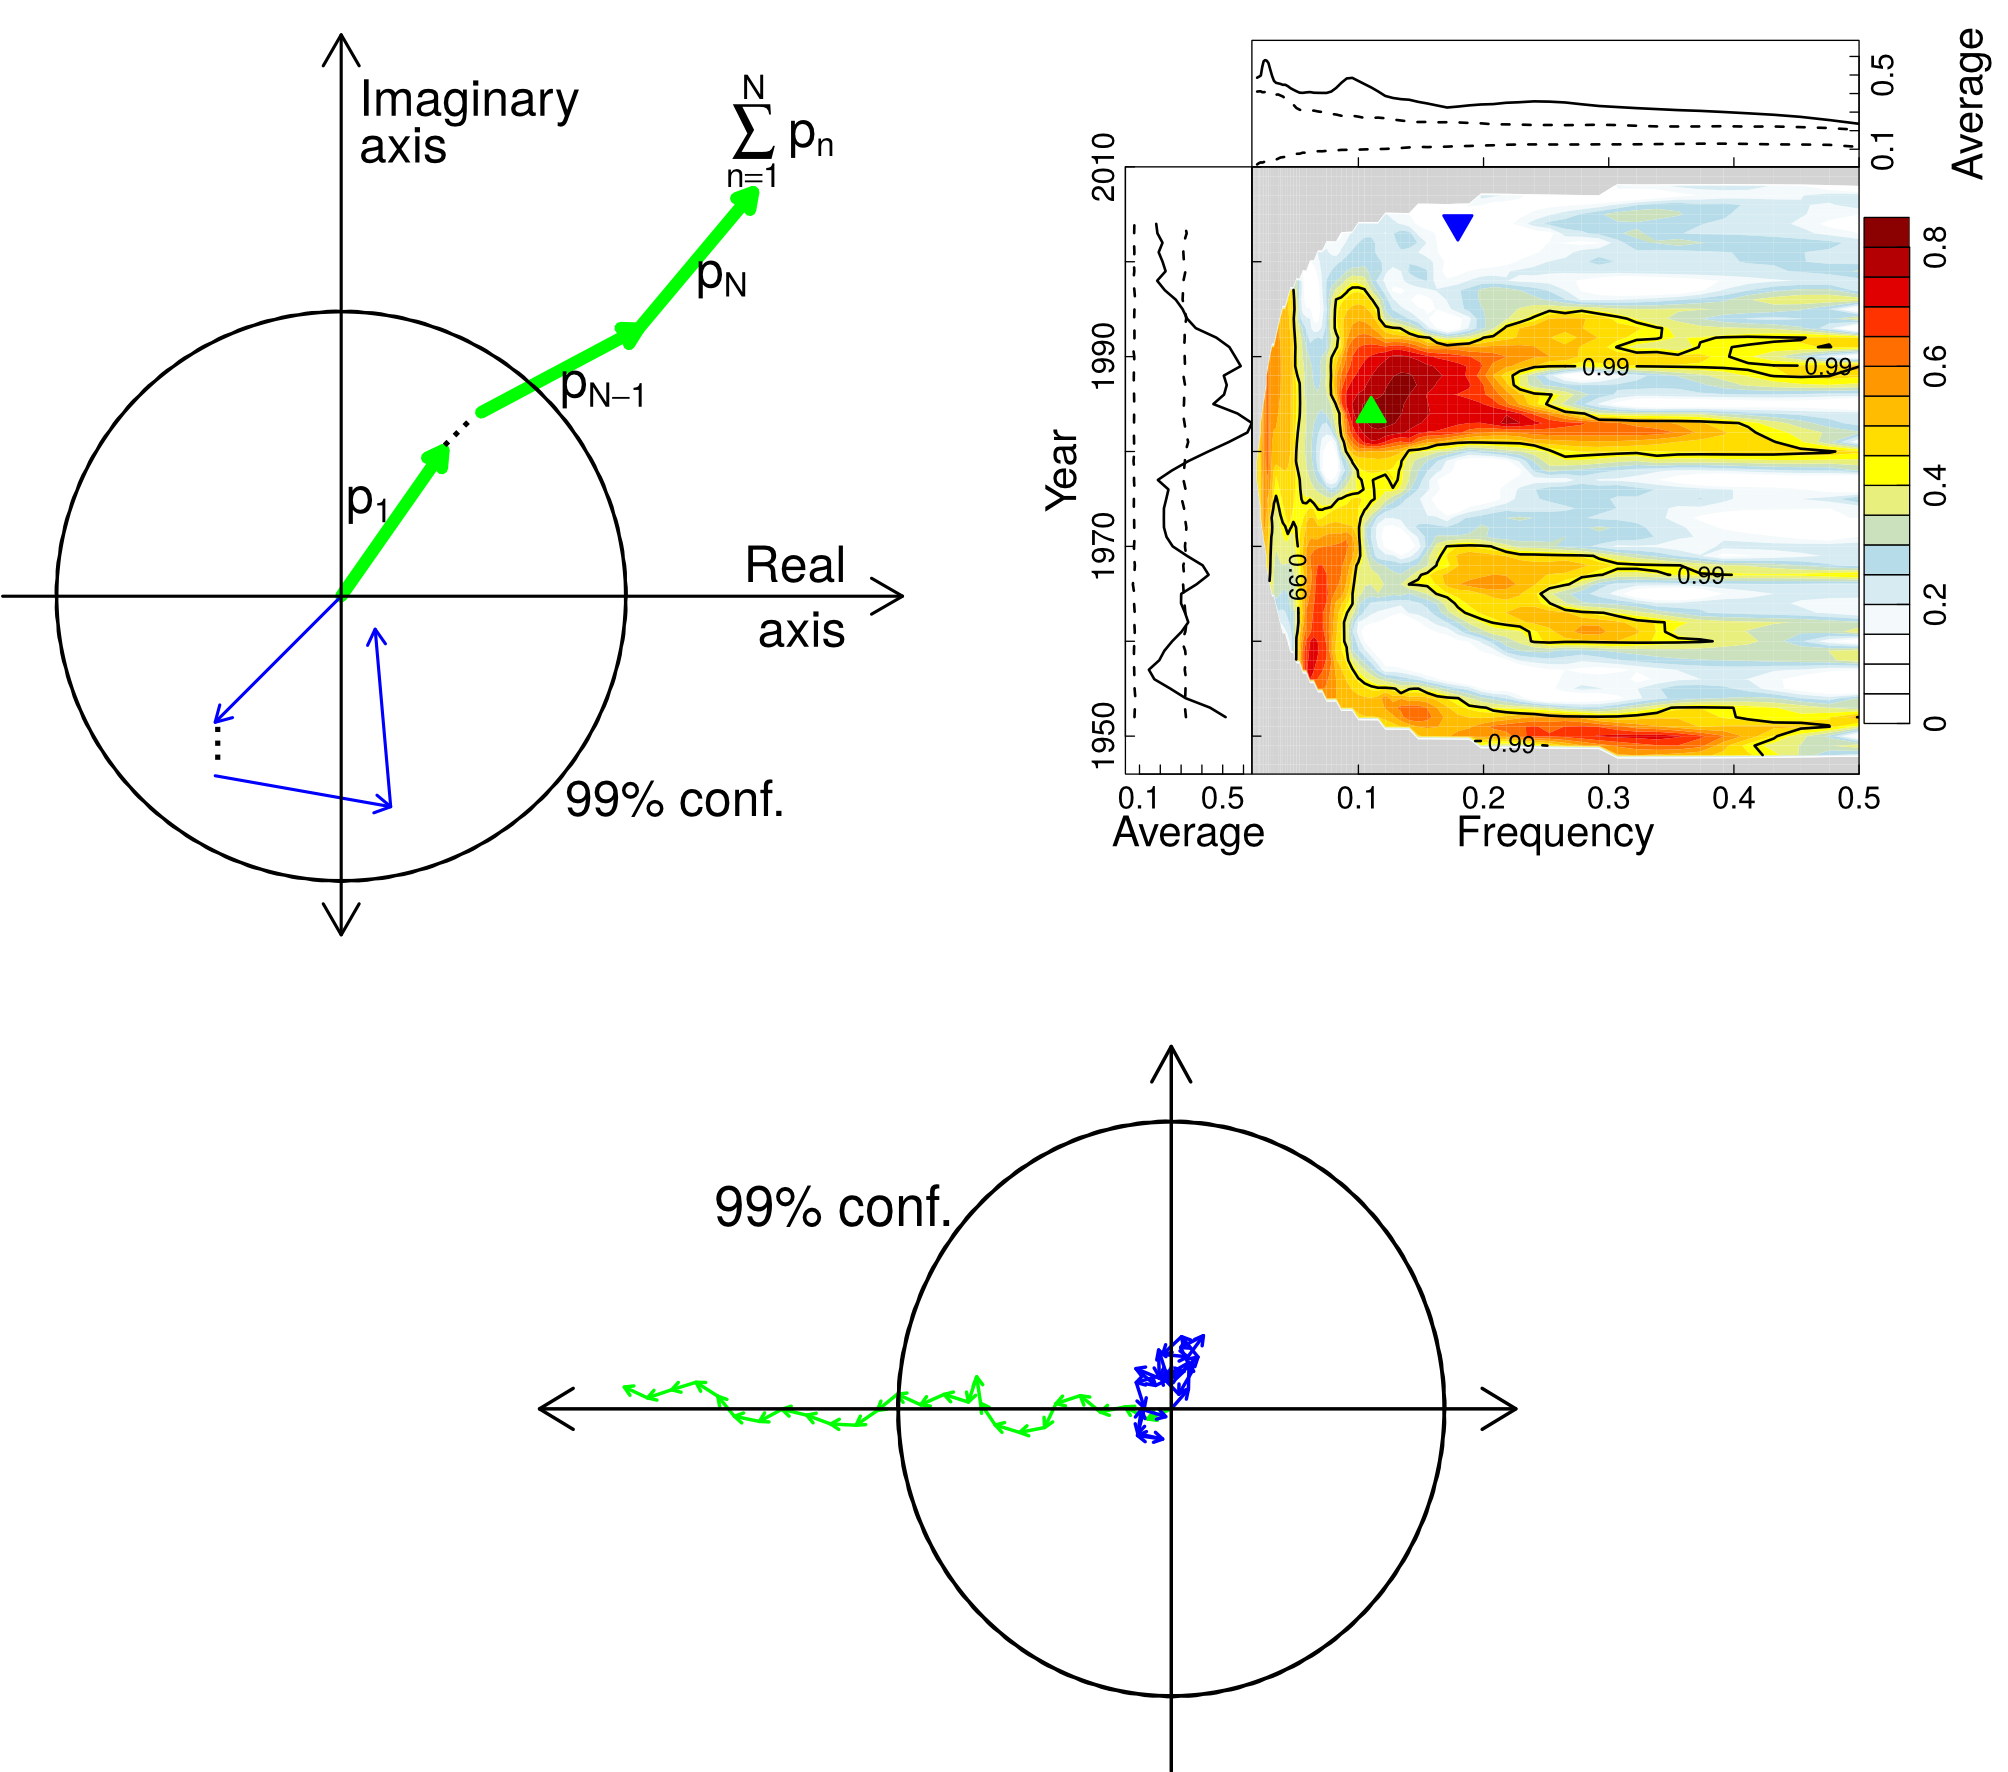
\includegraphics[height=8cm]{./figures/WPMF.png}
  \end{center}
\end{frame}

\begin{frame}[fragile]
\frametitle{Example of the wpmf: make some data}
\begin{block}{Fake data characteristics}
\begin{itemize}
\item Several time series
\item All have one underlying signal, switches from period 10 to 5 mid way
\item All have randomly phase-shifted period-3 sine ways
\item Plus white noise, independent in each signal
\end{itemize}
\end{block}
\end{frame}

\begin{frame}[fragile]
\frametitle{Example of the wpmf: make some data}
\begin{exampleblock}{Make some fake data}
\begin{verbatim}
times1<-0:50; times2<-51:100; times<-c(times1,times2)
ts1<-c(sin(2*pi*times1/10),sin(2*pi*times2/5))+1.1 

dat<-matrix(NA,11,length(times))
for (counter in 1:dim(dat)[1])
{
  ts2<-3*sin(2*pi*times/3+2*pi*runif(1))+3.1
  ts3<-rnorm(length(times),0,1.5)
  dat[counter,]<-ts1+ts2+ts3    
}
dat<-cleandat(dat,times,1)$cdat
\end{verbatim}
\end{exampleblock}
\end{frame}

\begin{frame}
\frametitle{Can you see synchrony in these data? Not really.}
\includegraphics[width=.49\textwidth]{../results/synthetic_results/WPMFExample_timeseries.pdf}
\includegraphics[width=.49\textwidth]{../results/synthetic_results/WPMFExample_PairwiseCorrelation.pdf}
\end{frame}

\begin{frame}[fragile]
\frametitle{Example of wpmf: apply \texttt{wsyn::wpmf}}
\begin{exampleblock}{Apply \texttt{wpmf}}
\begin{verbatim}
wpmfres<-wsyn::wpmf(dat,times,sigmethod="quick")
\end{verbatim}
\end{exampleblock}
\begin{block}{Notes}
\begin{itemize}
\item \texttt{wpmfres} is an S3 class defined for wpmfs 
\item Default values for other arguments are good for exploration, see docs and vignette for details
\end{itemize}
\end{block}
\end{frame}

\begin{frame}[fragile]
\frametitle{Example of wpmf: what do you get?}
\begin{exampleblock}{Plot magnitude}
\begin{verbatim}
wsyn::plotmag(wpmfres,sigthresh=0.95)
\end{verbatim}
\end{exampleblock}
\begin{columns}[c]
\begin{column}{6cm}
\includegraphics[width=\textwidth]{../results/synthetic_results/WPMFExample_wpmf.pdf}
\end{column}
\begin{column}{6cm}
\begin{itemize}
\item We get significant synchrony at timescale 10, initially, then at timescale 5
\item So we detect the time- and timescale-specific synchrony that was built into the data
\end{itemize}
\end{column}
\end{columns}
\end{frame}

\begin{frame}
\frametitle{Significance of the wpmf}
\begin{itemize}
\item Null hypothesis: random, independent phasors
\item Significance means phasors are significantly more aligned than that
\item Note: as always, you need to keep multiple testing in mind
\end{itemize}
\begin{center}
\includegraphics[width=.5\textwidth]{../results/synthetic_results/WPMFExample_wpmf.pdf}
\end{center}
\end{frame}

\begin{frame}
\frametitle{The wavelet mean field (\texttt{wsyn::wmf})}
  \begin{itemize}
    \item We also use the ``wavelet mean field'' $r_\sigma(t)=\frac{1}{N}\sum_{n=1}^{N}w_{n,\sigma}(t)$
    \item Where $w_{n,\sigma}(t)=W_{n,\sigma}(t)/\sqrt{\frac{1}{NT}\sum_{n=1}^{N}\sum_{t=1}^{T}W_{n,\sigma}(t)W_{n,\sigma}^{*}(t)}$ is a normalized wavelet transform
    \item The wmf uses magnitude as well as phase information, gives more complete information but a bit more complicated
    \item Can interpret it in a similar way
    \item But no straightforward significance testing!
    \item We often show both
    \item See \texttt{wsyn} vignette for details on how to call the \texttt{wmf} function
  \end{itemize}
\end{frame}

{\setbeamercolor{background canvas}{bg=lightgreen}
\begin{frame}
\frametitle{Benefits of a timescale-specific approach to synchrony so far}
\begin{itemize}
\item The example shows some benefits to a time/timescale-specific approach over classic correlation-based methods
\item Correlation methods did not show synchrony, since those methods conflated timescales and averaged across time
\item Synchrony on some timescales was obscured by asynchrony on others
\item We can now see the synchrony and see its structure
\item It turns out that timescale structure is very common in synchrony
\item It turns out that changes through time are also common, and a consequence of climate change
\end{itemize}
\end{frame}}

\subsection{Wavelet coherence}

{\setbeamercolor{background canvas}{bg=lightpink}
\begin{frame}
\frametitle{Starting to explore causes of synchrony}
\begin{itemize}
\item We know that one important cause of synchrony is the Moran effect
\item How do we start to explore that in a time/timescale-specific viewpoint?
\item We need to understand relationships between two sets of time series measured in the same places
(usually one environmental and one biological)
\item So data now consist of two sets of time series measured at the same times and places
\item Our approach is based on ``wavelet coherence''
\end{itemize}
\end{frame}}

\begin{frame}
\frametitle{The basic idea of wavelet coherence, by analogy}
\begin{itemize}
\item Our method will 
\begin{itemize}
\item quantify the consistency of the phase relationship between signals, through space and time
\item and compare that to what would be expected if the signals were unrelated but each had the same degree of phase drift across space and time
\end{itemize}
\item It is the very irregularity of biological time series that makes this method work
\item Clock analogy
\end{itemize}
\end{frame}

\begin{frame}
\frametitle{Spatial wavelet coherence}
\begin{itemize}
\item \texttt{wsyn} has a spatialized wavelet coherence tool to detect relationships between variables in a timescale-specific way
\item $w_{n,\sigma}^{(1)}(t)$ and $w_{n,\sigma}^{(2)}(t)$ normalized wavelet transforms
\item $w_{n,\sigma}^{(1)}(t) (w_{n,\sigma}^{(2)}(t))^{*}$ has phase equal to the phase difference
\item $\frac{1 }{NT}\sum_{n= 1}^{N}\sum_{t=1}^{T} w_{n,\sigma}^{(1)}(t) (w_{n,\sigma}^{(2)}(t))^{*}$ measures consistency of phase differences across time and location 
\item This sum is large when phase differences are consistent across space and time...
\item and small when they are not consistent
\item We compare against the same thing calculated for randomized ``surrogate'' datasets
\end{itemize}
\end{frame}

\begin{frame}[fragile]
\frametitle{Example of spatial coherence tools: make some data}
\begin{block}{Fake data characteristics: environmental data}
\begin{itemize}
\item Data consist of an environmental driver and a biological variable, both measured at $11$ locations
\item The environmental variable is the sum of:
\begin{itemize}
\item a weak common signal, period $10$
\item a strong common signal, period $3$
\item white noise 
\end{itemize}
\end{itemize}
\end{block}
\begin{exampleblock}{Make the fake environmental data}
\begin{verbatim}
times<-(-3:100); lt<-length(times)
ts1<-sin(2*pi*times/10)
ts2<-5*sin(2*pi*times/3)
x<-matrix(ts1+ts2,11,lt,byrow=TRUE)+
  matrix(rnorm(11*lt,0,1.5),11,lt)
\end{verbatim}
\end{exampleblock}
\end{frame}

\begin{frame}[fragile]
\frametitle{Example of spatial coherence tools: make some data}
\begin{block}{Fake data characteristics: biological data}
\begin{itemize}
\item population time series were the 3-step moving average of the environment 
\item plus white noise
\end{itemize}
\end{block}
\begin{exampleblock}{Make the fake biological data}
\begin{verbatim}
times<-0:100; lt<-length(times)
y<-matrix(NA,11,lt) #the driven (biological) variable
for (i in 1:101) {
  y[,i]<-apply(FUN=mean,X=x[,i:(i+2)],MARGIN=1) }
y<-y+matrix(rnorm(11*lt,mean=0,sd=3),11,lt)
\end{verbatim}
\end{exampleblock}
\end{frame}

\begin{frame}
\frametitle{Can you see the relationships here using ordinary correlation? Not really.}
\begin{columns}[c]
\begin{column}{5cm}
\begin{itemize}
\item For each location we computed the correlation between the biological and environmental time series
\item This is a histogram of those values
\item You can't really see any tendency toward correlation
\item Why?
\end{itemize}
\end{column}
\begin{column}{7cm}
\includegraphics[width=\textwidth]{../results/synthetic_results/CoherenceExample_LocalBiolEnvCorrs.pdf}
\end{column}
\end{columns}
\end{frame}

\begin{frame}[fragile]
\frametitle{Example of spatial coherence: apply \texttt{wsyn::coh}}
\begin{exampleblock}{Apply \texttt{coh}}
\begin{verbatim}
cohres<-wsyn::coh(dat1=x,dat2=y,times=times,
  norm="powall",sigmethod="fftsurrog1",
  nrand=1000,f0=0.5,scale.max.input=28)
\end{verbatim}
\end{exampleblock}
\begin{block}{Notes}
\begin{itemize}
\item \texttt{cohres} is an S3 class defined for holding coherence results
\item \texttt{nrand} is the number of bootstrapped (surrogate) datasets to use
\item see vignette for additional details
\end{itemize}
\end{block}
\end{frame}

\begin{frame}[fragile]
\frametitle{Example of coherence: what do you get?}
\begin{columns}[c]
\begin{column}{6cm}
\begin{itemize}
\item Coherence between environmental and population data is the red line
\item It is weak at short timescales (period 3) because of the moving average
\item It is strong at long timescales
\item Black lines are confidence thresholds based on surrogates, $95$ and $99\%$
\end{itemize}
\end{column}
\begin{column}{6cm}
\includegraphics[width=\textwidth]{../results/synthetic_results/CoherenceExample_PlotCoh1.pdf}
\end{column}
\end{columns}
\end{frame}

\begin{frame}[fragile]
\frametitle{Example of coherence: what do you get?}
\begin{columns}[c]
\begin{column}{6cm}
\begin{itemize}
\item Even though the period-3 environmental oscillation is much stronger than the period-10 ...
\item It does not influence the populations because of the averaging
\item Pop-env relationship depends on timescale!
\item You have to account for that if you want to detect it!
\item This will also influence the potential for Moran effects
\end{itemize}
\end{column}
\begin{column}{6cm}
\includegraphics[width=\textwidth]{../results/synthetic_results/CoherenceExample_PlotCoh1.pdf}
\end{column}
\end{columns}
\end{frame}

\begin{frame}[fragile]
\frametitle{Example of coherence: what do you get?}
\begin{columns}[c]
\begin{column}{6cm}
\begin{itemize}
\item You can also get the rank of the coherence compared to surrogate coherences
\item The timescales where this exceed the threshold are ``significant''
\item Keep in mind multiple-testing errors though
\end{itemize}
\end{column}
\begin{column}{6cm}
\includegraphics[width=\textwidth]{../results/synthetic_results/CoherenceExample_PlotRanks.pdf}
\end{column}
\end{columns}
\end{frame}

\begin{frame}[fragile]
\frametitle{Example of coherence: what do you get?}
\begin{columns}[c]
\begin{column}{4cm}
\begin{itemize}
\item \texttt{wsyn} can also compute $p$-values for particular timescale bands
\item Here we consider the timescale bands 2-4 and 8-12
\item This can help address multiple testing problems
\item See vignette for details
\end{itemize}
\end{column}
\begin{column}{8cm}
\includegraphics[width=\textwidth]{../results/synthetic_results/CoherenceExample_PlotCoh2.pdf}
\end{column}
\end{columns}
\end{frame}

\begin{frame}
\frametitle{Technical slide: Significance - what are these surrogates I mentioned?}
\begin{itemize}
\item Given data $x_n(t)$, $y_n(t)$, $n=1,\ldots,N$, $t=1,\ldots,T$
\item Compute the spatial wavelet coherence (a function of frequency/timescale)
\item Compute surrogates $x'_n(t)$, recompute spatial wavelet coherence for the surrogates
\item Repeat 10000 or so times
\item Compare coherence plot using data to the distribution of plots using surrogates
\end{itemize}
\end{frame}

\begin{frame}
\frametitle{Technical slide: Significance - what are these surrogates I mentioned?}
\begin{itemize}
\item Surrogates $x'_n(t)$ should have the same spatial and temporal autocorrelation properties as $x_n(t)$, but be unrelated to $y_n(t)$
\item How to get them (concept)
\begin{itemize}
\item Fourier transform all $x_n(t)$
\item Randomize the phases of the transforms, uses the same randomizations for all $n$
\item Reverse transform to get $x'_n(t)$
\end{itemize}
\item We have a fast algorithm: Sheppard et al (2017, EPJ, Nonlin Biomed Phys)
\end{itemize}
\end{frame}

{\setbeamercolor{background canvas}{bg=lightgreen}
\begin{frame}
\frametitle{Advantages of the timescale specific approach}
\begin{itemize}
\item Time series can be related to each other on some timescales and not on others
\item E.g., if moving average processes are what make them related
\item If you look for correlations, you might not see the relationship - lack of relationship on other timescales obscures the relationship that does occur on certain timescales
\item Coherence can fix that problem
\item Timescale specific relationships should be common in biology
\end{itemize}
\end{frame}}

\subsection{Attributing synchrony to causes}

{\setbeamercolor{background canvas}{bg=lightpink}
\begin{frame}
\frametitle{OK, how do we get from here to saying something about environmental causes of synchrony?}
\begin{itemize}
\item How does coherence relate to possible causative relationships?
\item How do we attribute synchrony to particular causes? 
\item What about interactions between causes?
\end{itemize}
\end{frame}}

\begin{frame}
\frametitle{Coherence can gives you information about causes of synchrony}
\begin{itemize}
\item Making claims about causes from observational data is fraught, but there are already several statistical frameworks for doing it
\item Our framework gives another that applies to environmental causes of synchrony
\end{itemize}
\end{frame}

\begin{frame}
\frametitle{Coherence can gives you information about causes of synchrony}
\begin{itemize}
\item If A is an environmental variable and B is a population variable, and A and B are highly significantly
coherent on a certain timescale band, then, logically, EITHER...
\begin{itemize}
\item A is driving B on that band, possibly indirectly OR
\item B is driving A on that band (very unlikely in this context) OR
\item They are mutually influencing each other (B-to-A influence very unlikely) OR
\item Some third variable C is driving both, or driving B and mutually related to A
\end{itemize}
\item In that case C is very likely another environmental variable
\end{itemize}
\end{frame}

\begin{frame}
\frametitle{Coherence can gives you information about causes of synchrony}
\begin{itemize}
\item So if A is an environmental variable and B is a population variable...
\item and A and B are highly significantly coherent on a certain timescale band...
\item and if A is synchronous...
\item Then we can reasonably claim to have identified a Moran effect
\item Can we then quantify how much synchrony in B is explained by synchrony in A?
\item Yes!
\end{itemize}
\end{frame}

\begin{frame}
\frametitle{Some analytic frameworks}
\begin{itemize}
\item Based on what I showed you, and for the purpose of understanding environmental drivers of synchrony...
\item We developed a wavelet linear modeling framework
\item And a ``wavelet Moran theorem'' and ``synchrony attribution theorem''
\item See Sheppard et al (2016), Nature Climate Change
\item And Sheppard et al (2019), Plos Comp Biol
\item And the vignette
\item I want to demo these tools with made-up data before Jon applies them
\item They provide a reasonably comprehensive tool set for investigating environmental causes of synchrony
\end{itemize}
\end{frame}

\begin{frame}
\frametitle{The made-up data: environmental}
\begin{itemize}
\item Everything is in 10 locations
\item Environmental variable 1, d1
\begin{itemize}
\item an oscillation of period $12$ years and an oscillation of period $3$ years
\item and strong white noise
\end{itemize}
\item Environmental variable 2, d2, was the same structure, but independently generated
\item Environmental variable 3, dirrel, was white noise only
\end{itemize}
\end{frame}

\begin{frame}
\frametitle{The made-up data: populations}
\begin{itemize}
\item The population in each location is influenced by the two drivers...
\item And by separate, independent local variability
\item Driver 1 is averaged over 3 time steps in its influence, so
only the period-12 variability in driver 1 influences the populations
\item Driver 2 influences populations directly
\item dirrel has no influence (hence the name)
\end{itemize}
\end{frame}

\begin{frame}
\frametitle{The goal}
\begin{itemize}
\item If we did not know the setup and only had the data, could we infer causes of synchrony?
\item Because of how the data were constructed, we know:
\begin{itemize}
\item d1 is important for synchrony on long timescales (12 years)
\item d2 is important for synchrony on long (12 years) and short (3 years) timescales
\item dirrel is not important for synchrony
\end{itemize}
\item Can we infer these facts from the data?
\end{itemize}
\end{frame}

\begin{frame}[fragile]
\frametitle{First fit a wavelet linear model}
\begin{exampleblock}{Use \texttt{wsyn::wlm}}
\begin{verbatim}
dat<-list(pops=pops,d1=d1,d2=d2,dirrel=dirrel)
wlm_all<-wsyn::wlm(dat,times,resp=1,pred=2:4,
  norm="powall",scale.max.input=28)
\end{verbatim}
\end{exampleblock}
\begin{block}{Wavelet linear model}
\begin{itemize}
\item $w^{(\text{pop})}_{n,\sigma}(t) = \alpha(\sigma) w^{(1)}_{n,\sigma}(t)+
\beta(\sigma) w^{(2)}_{n,\sigma}(t)+
\gamma(\sigma) w^{(\text{irrel})}_{n,\sigma}(t)$
\item See Sheppard et al (2019), Plos Comp Biol for details
\end{itemize}
\end{block}
\end{frame}

%slides that show the process of testing each variable to then drop dirrel
%then some stuff about calculating synchrony explained on each band
%then compare with what we know b/c of how the data were generated
%then a summay slide like "the point is, if you have the data, we can do X, Y Z"

\section{Kelp example}

\begin{frame}
\frametitle{Empirical example: kelp wrack on beaches near Santa Barbara, CA}
Goals for the empirical example:
\begin{itemize}
\item Add concreteness through application to a real question
\item Discuss some challenges posed by real-world data for application of methods
\end{itemize}
\end{frame}

\begin{frame}
\frametitle{Empirical example: kelp wrack on beaches near Santa Barbara, CA}
\begin{itemize}
\item Giant kelp (Macrocystis pyrifera) is a rocky reef foundation species
\item Its detritus provides a major resource subsidy to sandy beaches
\item Can kelp forest synchronize beach dynamics through provision of wrack?
\end{itemize}
\begin{block}{Reference}
Walter, J.A., et al. (2024) Spatial synchrony cascades across ecosystems and up food webs via resource subsidies. \textit{PNAS} 122(2) e2310052120.
\end{block}
%TODO add pretty pictures
\end{frame}

\begin{frame}
\frametitle{Data sources}
\begin{block}{Beach data}
Santa Barbara Coastal LTER, J. Dugan, SBC LTER: Beach: Time-series of beach wrack cover and biomass, ongoing since 2008 ver 16. Environmental Data Initiative (2021). \url{https://portal.edirepository.org/nis/mapbrowse?packageid=knb-lter-sbc.40.16}.
\end{block}
\begin{block}{Kelp forest and wave data}
T. Bell, SBC LTER: Reef: California kelp canopy and environmental variable dynamics ver 1.
Environmental Data Initiative (2023). \url{https://doi.org/10.6073/pasta/c40db2c8629cfa3fbe80fdc9e086a9aa}.
\end{block}
\end{frame}

\begin{frame}
\frametitle{Preparing data for analysis}
\begin{itemize}
\item Analyses in \texttt{wsyn} require complete, regularly spaced time series
\item Organize into site (beaches) by time (months, Jan. 200X to Dec. 20XX) matrices
\item Fill any gaps with beach- and month-specific medians
\end{itemize}
\end{frame}

\begin{frame}
\frametitle{Responsible gap-filling for synchrony analyses}
\begin{itemize}
\item Avoid borrowing information from neighboring sites. This can build in artefactual synchrony.
\item Be cautious with temporal structures---preserve things that have well-defined periods and consistent amplitudes, e.g., seasonal and diurnal cycles.
\item It may be impossible to responsibly fill many/large gaps. We have generally avoided analyzing time series with more than 20\% or so missing values, when there are several consecutive missing values, and when many/all locations are missing data simultaneously.
\end{itemize}
\end{frame}

\begin{frame}[fragile]
\frametitle{Data prep with \texttt{wsyn::cleandat}}
\begin{itemize}
\item \texttt{wsyn} requires each time series have mean = 0 and will throw an error if this is not the case.
\item May also detrend (linear), tranform to improve normality (Box-Cox), standardize (Z-score). 
\item Standard options provided in \texttt{cleandat}; controlled using \texttt{clev} argument.
\end{itemize}
\begin{exampleblock}{Apply \texttt{wsyn::cleandat}}
\begin{verbatim}
wrack <- as.matrix(read.csv("../data/wrack.csv"))
wrack.cln <- cleandat(wrack, tt, clev=5)$cdat 
\end{verbatim}
\end{exampleblock}
\end{frame}

\begin{frame}[fragile]
\frametitle{Make \texttt{wmf} and \texttt{wpmf}}
%\begin{exampleblock}{Apply \texttt{wsyn::wmf} and \textt{wsyn::wpmf}}
%\begin{verbatim}
%wmf.wrack <- wsyn::wmf(wrack.cln, tt)
%wpmf.wrack <- wsyn::wpmf(wrack.cln, tt, sigmethod="quick")
%wsyn::plotmag(wmf.wrack)
%wsyn::plotmag(wpmf.wrack)
%\end{verbatim}
%\end{exampleblock}
\end{frame}

\begin{frame}
\frametitle{Interpret wmf and wpmf}
%TODO add images
%Remember to talk here about choosing timescale bands to focus on
\end{frame}

\begin{frame}
\frametitle{Coherence testing}

\end{frame}


\begin{frame}

\end{frame}

\end{document}